\section{State of the art on silicon-level investigation}

In previous sections, major \gls{esd} standards used in laboratories were presented.
The impact of electrostatic discharges on electronic devices has been detailed, highlighting two classes of failures.
Hard-failures are well known and multiple protection strategies exists, from external devices and ESD protections, to distributed protection architectures and much more.
Soft-failures are the kind of issue caused by electrical fast transients.
When discharges propagate inside electronic equipments and reach integrated circuits, they can cause them to malfunction.
For multiple reasons described in previous sections, it is essential to detect early functionnal weaknesses.
This section is a review the litterature of the current state of the art on \gls{esd} induced soft-failure analysis.
Study cases, observation methods and modeling approaches are presented.

\subsection{Case studies}

% Case 1 - NXP bandgap + substrate coupling
K. Abouda details in \cite{softfailEMCIC} a case of soft-failure on an integrated automotive regulator \gls{ic}.
The failure signature is a loss of the regulated voltage when exposed to \gls{bci} ISO11452-4 \cite{iso11452}.
The test setup is provided in Fig. \ref{}.
The product is investigated manually, by searching inside the design for coupling and propagation paths, and performing multiple simulations.
Eventually, it was proven that a residue of the disturbance was coupling through the substrate on a current mirror inside the bandgap reference.
During the disturbance, bandgap voltage was shifting from its nominal value.
After some delay, the bandgap output was reaching an undervoltage threshold, causing the entire system to restart.
To avoid it, a design fix was proposed by filtering at the appropriate spot inside the design to avoid the amplification of the disturbance.

\begin{figure}[!h]
  \centering
  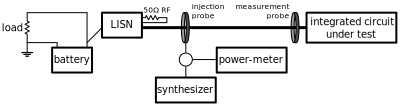
\includegraphics[width=\textwidth]{src/1/figures/bci_setup.pdf}
  \caption{Bulk Current Injection setup}
  \label{fig:bci-setup}
\end{figure}

% Case 2 - CESAME IC - paper Vrignon + Ben dhia
N. Lacrampe presents another failure case in \cite{LacrampeTransientImmunity}.
Very-fast \gls{tlp} is injected on an 0.18 \textmu{}m CMOS technology (1.8 V supply voltage) testchip.
The chip contains 6 instances on the same logic core, differing only by their power-rails architecture.
The injection on power rails is performed using a \gls{dc} block 1 nF capacitor, similarly to the \gls{dpi} standard \cite{iec62132-4}.
% What is the failure signature
An output signal of the logic core is monitored.
The susceptibility criteria is the amplitude crossing a 20\% threshold from the established logic level.
Above this threshold, the core is supposed to no longer work reliably.
It is proven that modelling the output buffer of the core logic is enough for reproducing with less than 20\% error the waveform on the output.
It is less accurate than a full-netlist simulation, but faster to simulate.
VHDL-AMS and \gls{spice} modelling are performed in this analysis.

%TODO: Pictures
% Case 3 - failures on an SDRAM
%TODO: Read reference articles in this article
In \cite{SDRAMCase}, soft-failures are studied on a SDRAM memory in operation.
The injection setup consists of a modified compact \gls{tem} cell \ref{fig:modified-tem-cell} with a reduced septum height.
Reduced dimensions result in increased field strenghts, to reach levels normally produced by an \gls{esd} gun.
The discharge waveform, injected inside the cell, is generated by a filtered \gls{tlp} and is similar in shape to IEC 61000-4-2 \cite{iec61000-4-2}.
The SDRAM chip is mounted on a board.
Data is written and read on the memory by \gls{fpga}.
Differences between incoming and outgoing data signifies a functional failure of the memory.
Only the memory is exposed to the disturbance, the rest of the board's devices are located outside of the \gls{tem} cell, on the other side of the board.
The main defect of this method is to only provide a global failure level.
It does not allow to identify which particular net or pin is the most sensitive to disturbances.

\begin{figure}[!h]
  \centering
  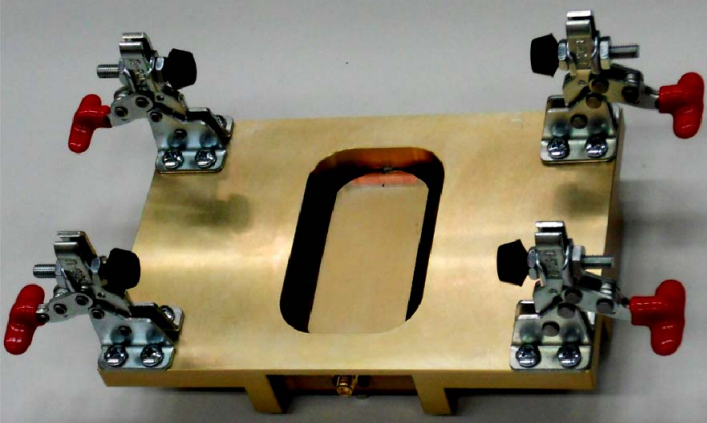
\includegraphics[width=0.6\textwidth]{src/1/figures/modified_tem_cell.png}
  \caption{Modified TEM cell from \cite{SDRAMCase}}
  \label{fig:modified-tem-cell}
\end{figure}

B. Orr reports in \cite{softFailSubsystem} errors caused by electrostatic discharges on two different camera communication buses.
Events of different severities are observed, depending on the discharge parameters.
It is attempted to determine whether the sensor or the application processor is causing the error.
The magnetic emission map is recorded with a near-field magnetic scanner to try to observe local variations in the emission spectrum because of the degradation of functionnality.
It was envisionned that soft-failure can induce significant variations in the emission spectrum of a disturbed component, and thus those variations could help localize them.
In this particular case, the root cause of failures could not be determined.

An LCD display is studied in \cite{softFailLCD}.
The device is tested with an IEC 61000-4-2 \cite{iec61000-4-2} generator, and non-destrutive problems are observed due to the discharge.
Electromagnetic disturbances cause stripes to appear on the display, optical parameters changes and blacklighting malfunctions.
System-level testing waveforms were found too complex for identifying the root cause.
A near-field injection is performed to identify which trace of the LCD's flex connector claims the lowest immunity.
The lack of resolution of the near-field probe caused multiple traces to be disturbed at once, preventing this second approach to work.
Finally, the individual track stressing was repeated with a capacitively-coupled \gls{tlp} on each individual metal track.
However, results were once more unconclusive and no metal trace could categorically be identified as more sensitive than the others.
The conclusion for this paper is that silicon level soft-error models are required for standard investigation.

An investigation method is presented in \cite{softFailMobile} to search for discharge propagation paths responsible for soft-failures on a mobile phone.
The IEC 61000-4-2 standard is chosen as testing waveform.
Metallic parts are assumed to be the main propagation paths.
To confirm this hypothesis, time-domain electromagnetic field 3D simulations of almost the entire phone are ran (see Fig. \ref{fig:mobile-phone-3d-em})
After the failure location was determined, RC-networks are used as countermeasures to protect physical inputs and outputs, like buttons, LCD inputs and connectors.

\begin{figure}[!h]
  \centering
  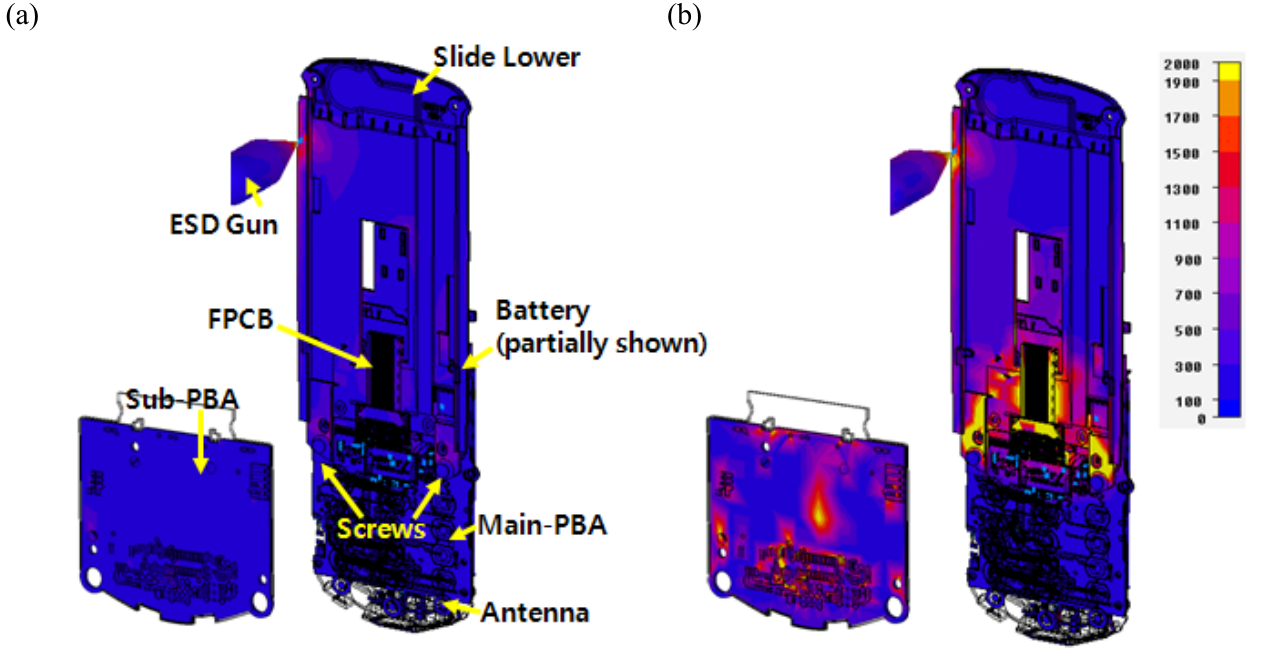
\includegraphics[width=0.8\textwidth]{src/1/figures/current_distribution_mobile.png}
  \caption{ESD Current Distribution on Mobile Phone and Backside sub-battery pack at (a) 1.0 ns and (b) 1.8 ns (Credit: \cite{softFailMobile})}
  \label{fig:mobile-phone-3d-em}
\end{figure}

\subsection{Observation methods}

F. Caignet proposes in \cite{eq-time-sampling} an on-chip measurement technique capable of recording \gls{esd} waveforms with a 20GHz bandwidth.
It relies on equivalent-time sampling for measuring waveforms with a much larger bandwidth that real-time oscilloscopes.
Equivalent time-sampling works exclusively with repeatable or periodic signals.
A real-time oscilloscope takes a complete waveform constituted of \textit{N} samples in a single shot.
On the other hand, a time-equivalent sampler measures waveforms point by point, and require \textit{N} repetitions of the waveform to acquire the \textit{N} samples.
The process for acquiring the data is the following.
A first waveform is shot, and the sampler only records its value at $t=0$.
A second waveform is shot, and the sampler records the value at $t=\Delta t$.
At the third waveform, the recording is at $t=2\Delta t$.
The process is repeated while increasing the sampling delay by \textDelta{}t at each step until enough points were acquired.
This approach is interesting because it reduces a lot the constraints on the measurement system, while offering a huge bandwidth.
The main disavantage is that it requires as many measurements as the amount of points needed.
In \cite{eq-time-sampling}, the sampler was designed using a CMOS 65nm technology and embedded into a testchip.
Architecture is given in Fig. \ref{fig:eq-time-sampler-architecture}.

\begin{figure}[!h]
  \centering
  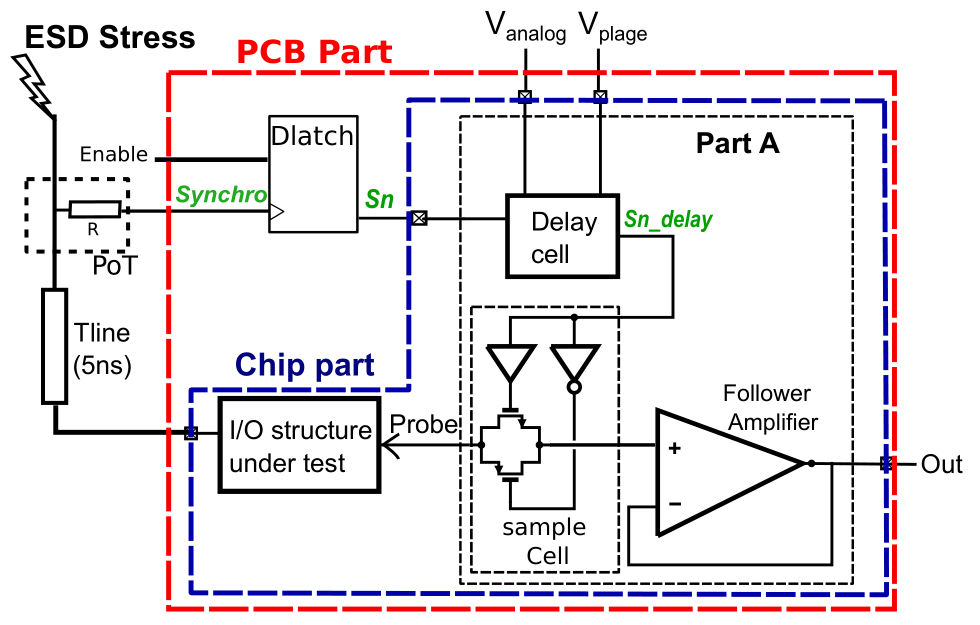
\includegraphics[width=0.6\textwidth]{src/1/figures/architecture_equivalent_time_sampler.png}
  \caption{Equivalent time-sampler architecture from \cite{eq-time-sampling}}
  \label{fig:eq-time-sampler-architecture}
\end{figure}

Other techniques exist in similar fields that could prove useful for ESD investigation.
M. Nagata details in \cite{substrate-noise-measurement} an on-chip measurement technique in for recording substrate noise waveforms at silicon level.
Injection and measurement structures are directly integrated into a 0.4\textmu{}m CMOS technology test vehicle.
The injection structures consists in a controllable noise source.
The amount of logic elements, transition directions and delays can be selected to generate different noise waveforms.
By coupling, the substrate receives a part of this disturbance.
The sensor consists in a latch comparator \ref{fig:noise-detect-latch-comparator}.
With a few synchronisation signals, it is sufficient to record waveforms with a 100ps time resolution.
For \gls{esd}, this sampling frequency is almost ideal.

\begin{figure}[!h]
  \centering
  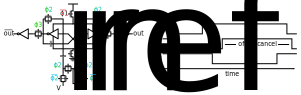
\includegraphics[width=\textwidth]{src/1/figures/latch_comparator.pdf}
  \caption{Latch comparator and timings for substrate noise detection from \cite{}}
  \label{fig:noise-detect-latch-comparator}
\end{figure}

%TODO ?
%\subsubsection{Optically-isolated communication}
%Banc Alain

\subsubsection{Emmission Microscopy (EMMI)}

% Concept
\gls{emmi} is an observation technique where a camera registers photon emission above semiconductor devices.
A device is placed in the field of view of the camera.
The entire system is placed inside an enclosure to block out all ambient light.
Semiconductor junctions and defects emit photons when electrically excitated.
By letting the camera shutter open for a long time, between a few hundred milliseconds to tens of seconds, photons generated by this process are detected by the image sensor.
As photons accumulate, some sections of the image become brighter than others.
Defects can be isolated from normal junctions by comparing recordings performed on tested devices with a reference device.
The architecture of an \gls{emmi} system is provided in Fig. \ref{fig:emmi}.

\begin{figure}[!h]
  \centering
  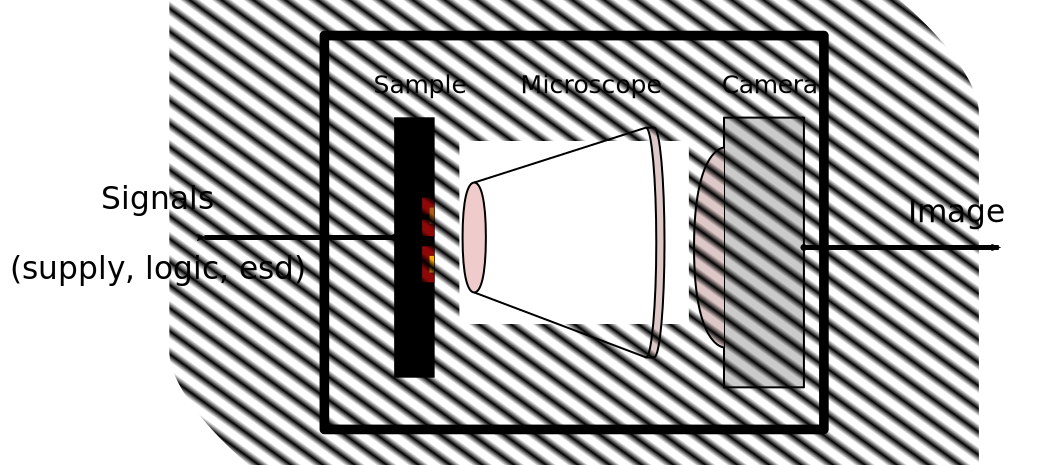
\includegraphics[width=0.8\textwidth]{src/1/figures/architecture_emmi.pdf}
  \caption{Architecture of an emission microscopy testbench}
  \label{fig:emmi}
\end{figure}

% In ESD field, how was used EMMI
Originally, the combination of \gls{emmi} with a \gls{tlp} discharge was proposed by T. Maloney and N. Khurana in the original TLP paper \cite{TLP}.
Afterwards, EMMI was employed for debugging hard-failures of ESD protections in 3D CMOS technologies \cite{kessler2002method} or high-voltage silicon technologies \cite{emmi-tlp}.
In US patent 6469536 \cite{kessler2002method}, Kessler describe a method to synchronize the ESD injection with the shutter of the EMMI.
Finally, \gls{emmi} is presented in \cite{softfailEMMI} as a successful analysis method for debugging and locating a functional failure on an integrated circuit exposed to \gls{esd}.
In this last paper, the integrated circuit is powered-on and in normal operation, and the \gls{emmi} helps localizing soft-failures.

% Show examples
Fig. \ref{fig:emmi-examples} shows two different images recorded with an \gls{emmi} bench.
The image on the left is the reference image and the one on the right is the signature after a failure.

\begin{figure}[!h]
  \centering
  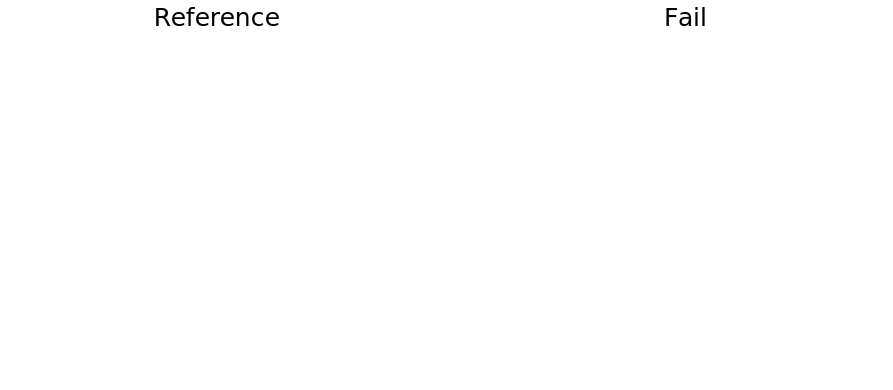
\includegraphics[width=\textwidth]{src/1/figures/emmi_comparison.pdf}
  \caption{reference and fail EMMI measurement of an integrated function}
  \label{fig:emmi-examples}
\end{figure}

\subsubsection{Near-field scanner}

% Introduce near-field scanner
Electromagnetic near-field scanner measure maps of electric and magnetic field.
An electric or magnetic probe is swept closely above a device to record the emitted field in near-field conditions.
Measurements may be carried out in the frequency domain or in the time domain.
This tool was initially intended for architectural analysis such as floor-planning and power distribution analysis.
For ESD, spatial information provided by the recorded map is very useful to locate failures and malfunctions.
A comprehensive and detailed analysis of near-field antennas is done by A.D. Yaghjian in \cite{nfsFirstStudy}.
More recent work details the principle of operation, data processing and hardware requirements in \cite{planarNFSAntenna, NFSMeasurements, NFScanner}.
Finally, measurement of electromagnetic emissions with surface scan method is standardized in IEC TS 61967-3 \cite{iec61967}.
The architecture of a near-field scanner is given in Fig. \ref{fig:near-field-scanner}.

\begin{figure}[!h]
  \centering
  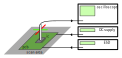
\includegraphics[width=0.4\textwidth]{src/1/figures/architecture_near_field_scanner.pdf}
  \caption{Architecture of a near-field scanning testbench}
  \label{fig:near-field-scanner}
\end{figure}

% Challenges
In a near-field scan, the amplitude recorded by the probe depends on many factors.
The amplitude measured from the sensor is the result of coupling between the source of emission and the sensor itself.
In the case of a magnetic sensor constituted of a loop, the size of the loop, the diameter of the wire, the orientation of the loop and the amount of turns all impact strongly the measured waveform.
Those characteristics can be estimated or measured.
However, the waveform also depends on other factors harder or impossible to determine.
For instance, the height between the emission source (usually a metal track) and the probe and the width of the track affect the coupling ratio.
For realistic integrated circuits, there can be a dense network of metal tracks that all will emit electromagnetic radiations and couple to the sensor.
It is impossible to measure each track independently.
Ultimately, determining absolute values of current or voltage inside a particular portion of an integrated circuit is nearly impossible.
This is why near-field scanners are more interesting for obtaining relative values between different sections of the circuit.
For instance, knowing that the magnetic field above a given structure is ten times greater than another structure is a precious information for understanding ESD propagation.

% Future work
So far, near-field scans are performed mostly at the \gls{pcb} level.
A new trend is to use scanners for integrated circuits.
In current silicon technologies, transistors are a few micrometers long, and metal tracks without power a few micrometers wide as well.
This range of dimensions is to compare with the capabilities of current near-field scanners.
Spatial resolution of a near-field scanner is not bounded by the 3-axis that moves the probe, but by the probe itself.
3-axis machines can easily be found with a positionnal accurary of a micrometer, less than the typical observable structure dimensions on silicon.
However, spatial resolution of current near-field probes is more in the range of 100\textmu{}m.
This value depends mainly on the size of the loop, its diameter and the distance between sensor and source.
For integrated circuits, this is not sufficient to isolate and identify structures.
In the future, improvements can be expected on the spatial resolution, but it will raise new kinds of challenges.
In the case of a probe with a resolution in the range of a 1\textmu{}m, the amount of points to records to build the map becomes huge.
For a 5mm by 5mm silicon circuit sampled every micrometer, scanning the entire area requires 2.5 million ESD pulse injection and recordings.
No integrated circuit can sustain such an amount of repeated stressing, and the device will be destroyed before the end of the scan.
Also, the test time for this brute force approach is going to be very important.
If the entire process is automated and a delay of 2 seconds is left between each point, the test campaign will still take 1388 hours, approximately 2 months.
Clearly, smarter sampling strategies to reduce this count or new measurement methods will be required before near-field scanning can be used for silicon-level investigation.

% Near-field scan as injection tool
So far, near-field scan has been presented as a measurement tool, but it can also serve as a localized stress injection system.
Instead of sensing voltage or current in the near-field probe, a pulse is injected in it.
In \cite{NearFieldInjectionFabrice}, a near-field scanner is combined with a very fast \gls{tlp}.
A stress is injected, and the device under test is monitored for faults.
A susceptibility map is obtained \ref{fig:near-field-scan-map}, that highlights the most sensitive areas of a board.
The paper demonstrates that it is possible to map quantitatively and with good resolution the \gls{esd} susceptibility of a board with this method.
In a similar approach, \gls{esd} sensitive metal tracks and \gls{ic} pins are identified in \cite{NearFieldInjectionBis} using a near-field scanner as an injection system.

\begin{figure}[!h]
  \centering
  \includegraphics[width=0.4\textwidth]{src/1/figures/near_field_scanner_susceptibility_map.pdf}
  \caption{Susceptibility map of a board recorded with surface scan in injection configuration \cite{}}
  \label{fig:near-field-scan-map}
\end{figure}


\subsection{Modeling methods of soft-failures for integrated circuits}

%TODO
Various methods presented in the litterature for ESD modelling
3D electromagnetic simulations, compact models, behavioral models, physically based models, linear vs non linear, etc have been evaluated.

% TODO
Mixed mode ESD simulations \cite{mixedModeESDSims}.
Combination of SPICE and TCAD models in an electrical simulation
Claims Using physical device models allows a higher accuracy and more realistic simulations than in comparison to when only behavioral SPICE based models are used.
On-chip and off-chip device interactions
Powered off and powered on behavior

% TODO
SEED methodology ? in \cite{usb2ESDProtection}.
Use TLP extracted I(V) curves to model both external protection and an IC pin.
Extraction of PCB model from layout.
Model is S-parameters
Interactions between all external devices and onchip devices.
Modelling approach is interesting for soft-failure analysis because it is thorough and enables accurate ESD simulation

% TODO
3D EM simulation \cite{LacrampeTransientImmunity} at silicon level, with the integrated circuit layout.
Aim is to predict susceptibility of integrated circuits against ESD
Deduce capacitive couplings between Vdd and Vss rails from layout + 3D EM simulation using HFSS (Ansoft) software
Model PCB tracks by distributed RLC
Model by equivalent impedance
Alternative to parasitic device extraction directly from layout.
IBIS package data was employed to model the package by an RLC equivalent
Modelling of a TLP stress generator using a lookup table I(V) component, in series with a 50\textOmega{} resistor.

% TODO
Electromagnetic fullwave simulations are conducted in \cite{softFailMobile}.
System-level components are simulated, such as PCB, metallic casing and battery back.
3D EM simulations highlighted main discharge paths and helped locate the failure

% IBIS is not enough for modelling an IC pin for ESD simulations
Input Output Buffer Information Specification (IBIS) \cite{ibis-spec} is a method for digital circuits providing the I/V characteristic of an IC without disclosing any circuit or process information.
IBIS provides a behavioral modeling technique for digital circuits for performing signal integrity simulation.
The idea is to characterize and distribute information about the package, buffers and protection diodes (not ESD protections), not the IC core.
It is demonstrated in \cite{ibisImprovementFabrice} that for EMC and ESD simulations the model is not sufficient.
It is not defined for fast impulses and high injection.
